%% grundlagen.tex
%% $Id: grundlagen.tex 28 2007-01-18 16:31:32Z bless $
%%

\chapter{Grundlagen}
\label{ch:Background}

Zunächst wir das Projekt \emph{TherapyBuilder} der Firma \emph{movisens GmbH} näher erläutert. Dies dient zum besseren Verständnis der Forschungsfrage und porträtiert die Rahmenbedingungen dieser Arbeit. Anschließend wird die Expertengruppe näher definiert. Des weiteren werden grundlegende Rahmenbedingungen ermittelt, die für Psychotherapien gelten. Abschließend wird die Definition eines Chatbots erläutert und erklärt, was unter einem Chatbot im Rahmen dieser Arbeit verstanden wird. 

\section{TherapyBuilder}

Das Projekt \emph{TherapyBuilder} entstand im Rahmen verschiedener Überlegungen der Firma \emph{movisens GmbH} .Die Firma \emph{movisens GmbH} bietet Produkte und Dienstleistungen für ambulantes Assessment in der Forschung an. Unter ambulantes Assessment wird hierbei das Erfassen von Daten einer untersuchten Person im Alltag verstanden. Ambulant bedeutet in diesem Zusammenhang, dass sich die Personen in ihrem natürlichen Umfeld im Alltag befinden. Für die Datenerfassung ist kein vorbestimmter Ort notwendig an dem sich der Proband stationär einfinden muss. Diese Erfassung kann über verschiedene Methoden geschehen. Eine Möglichkeit ist das Tracken von Patientenverhalten über verschiedene Sensoren. Diese können beispielsweise am Patienten selbst angebracht sein. Im Laufe der Datenerhebung zeichnen die Sensoren die benötigten Daten auf. Eine weitere Methode ist die \emph{Experience Sampling Method} (\emph{EMS}). Bei dieser Methode führt die zu untersuchende Person eine Art Tagebuch zur gezielten Selbstbeobachtung. Diese Methode kann heute leicht mit Hilfe von Smartphones umgesetzt werden.\cite{Assessme23:online} 

Das Produkt \emph{movisensXS} der Firma \emph{movisens GmbH} bietet bereits verschiedene Funktionen zur Umsetzung von Datenerhebung via \emph{EMS}. Mit diesem Tool können Forscher Fragebögen erstellen und sie auf den Smartphones ihrer Probanden ausführen lassen. Einige der bereits erstellten Fragebögen verwenden Dialoge in Form von Anleitungen, Fragen von Seiten des Forschers und den darauf folgenden Antworten des Probanden. Diese Fragebögen könnten von den Vorteilen eines Chatbots profitieren. So könnten die Nutzer eine höhere Zufriedenheit bei der Nutzung empfinden und eine größere Bereitschaft zeigen, die Fragebögen auszufüllen und Anleitungen durchzuführen (vgl. \cite{Fitzpatrick2017}). 

Da die derzeitige \emph{EMS}-Plattform \emph{movisensXS} noch keine Chatbot-ähnliche Ausgabe unterstützt, wurde das Projekt \emph{TherapyBuilder} gestartet. Ziel des TherapyBuilder-Projekts ist die Entwicklung eines Softwaretools, mit dessen Hilfe Anwender (medizinisch-therapeutische Experten) prototypische aber studientaugliche digitale Therapiesysteme erstellen können. Dies soll innerhalb weniger Tage mit minimalem finanziellen Einsatz und ohne Programmierkenntnisse realisierbar sein, um so die Wirksamkeit von Methoden und Therapieansätze in kürzester Zeit evaluieren zu können. Dabei soll das Projekt \emph{TherapyBuilder} derart gestaltet sein, dass der Anwender sich nicht um eine Medizinproduktegesetz (\emph{MPG})-konforme Softwareentwicklung kümmern muss. 

Das Projekt setzt sich aus den vier Komponentent \emph{Forscher-Plattform}, \emph{Therapeuten-Plattform}, \emph{Backend} und \emph{App} zusammen. Die Komponenten werden nachfolgend näher beschrieben.

\begin{figure}[h]
\centering
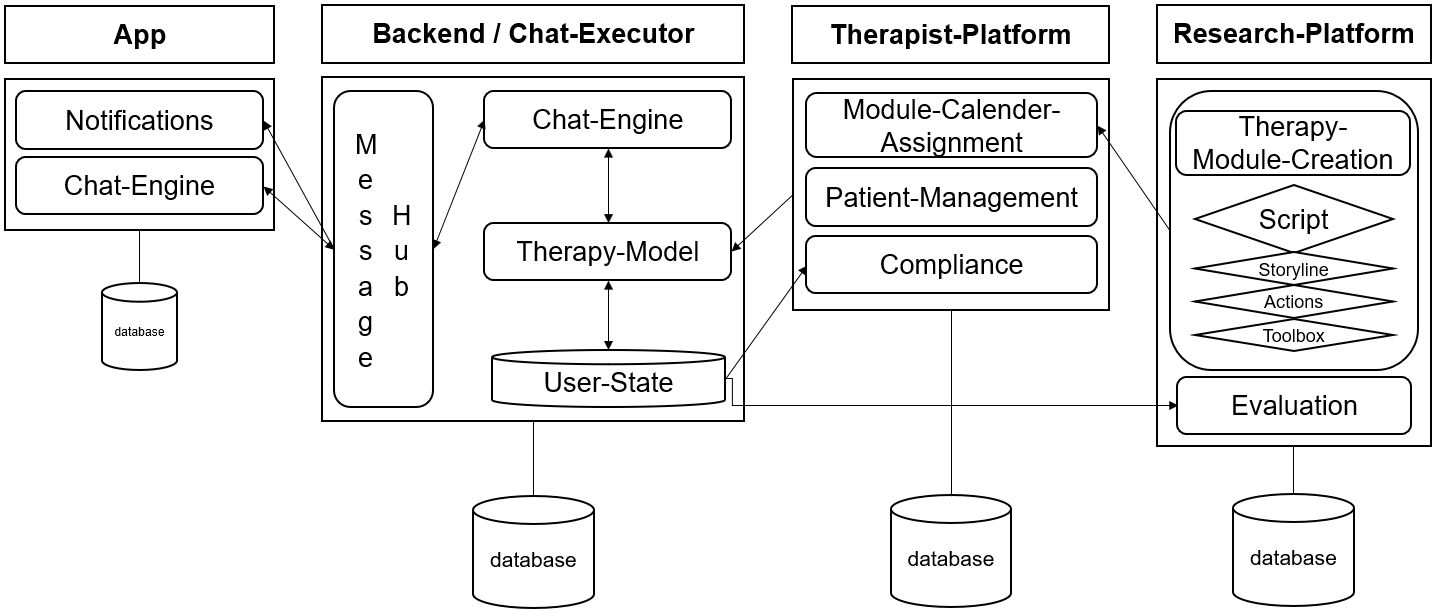
\includegraphics[width=1\textwidth]{pictures/TherapyBuilder}
\caption{Architektur des \emph{TherapyBuilders}}
\label{therapyBuilder}
\end{figure}


\subsection{Forscher-Plattform}

Auf dieser Plattform wird die Umsetzung eines studientauglichen digitalen Therapiesystems realisiert. Unter einem studientauglichen digitalen Therapiesystem wird ein System verstanden, welches zur Umsetzung von Therapien eingesetzt werden kann. Die Therapien werden in diesem Fall digital, beispielsweise über ein Smartphone, Tablet oder Computer, bereitgestellt. Die Therapie kann dabei in Form einer Studie evaluiert werden.

Die Forscher-Plattform erlaubt Forschern eine digitale Therapie anzulegen. Diese kann später über die Therapeuten-Plattform der entsprechenden Zielgruppe zugänglich gemacht werden. Eine Therapie setzt sich dabei aus verschiedenen Therapiemodulen zusammen. Ein Therapiemodul ist gleichbedeutend mit der Umsetzung einer Therapiemethode. Der Aufbau des Therapiemoduls lässt sich wie folgt versinnbildlichen.

Das Therapiemodul folgt einer Art Skript (\emph{engl. Script}). In diesem Skript wird festgelegt wann und auf welche Weise ein Dialog zwischen Anwender und Chatbot gestartet wird. Innerhalb des Skripts gibt es verschiedene Handlungsstränge (\emph{engl. Storylines}). Ein Handlungsstrang beschreibt einen Dialog zwischen Nutzer und Chatbot und dessen Verlauf. Der Handlungsstrang kann neben einem normalen Dialog auch aus verschiedenen Aktionen (\emph{engl. Actions}) bestehen, die dem Nutzer bereitgestellt werden um beispielsweise Tagebuch über verschiedene Verhaltensweisen zu führen. Auch kann ein Handlungsstrang Übungen beinhalten, die der Nutzer durchführt. Diese Übungen können dem Nutzer als Werkzeug in einer Art Werkzeugkasten (\emph{engl. Toolbox}) bereitgestellt werden. Somit kann der Nutzer jederzeit auf diese Übungen zugreifen.

Der in dieser Arbeit entwickelte \emph{TMA} wird später in dieser Plattform umgesetzt.  


\subsection{Therapeuten-Plattform}
Die Verwaltung der Patienten findet auf der Therapeuten-Plattform statt. Auf dieser können Patienten hinzugefügt, entfernt sowie verschiedene Therapiemodule ihren Profilen zugeteilt werden. Jedes Probandenprofil enthält eine Darstellung der aktuell zugeteilten und aktiven Therapiemodulen in Form eines Kalenders. Der Therapeut kann anhand dessen nachvollziehen, wie der entsprechende Therapieplan des Patienten aufgebaut ist. Außerdem kann hier auch das Einsehen des Therapiestands des Patienten ermöglicht werden. Die entsprechenden Profildaten werden in einer zugehörigen Datenbank gespeichert.


\subsection{Backend}



\subsection{App}



\section{Rahmenbedingungen von Psychotherapien}

\begin{itemize}
\item Intervention
\item Just in Time
\item Psychologischer Psychotherapeut
\item Experience Sampling
\end{itemize}

\section{Chatbots}

%https://wirtschaftslexikon.gabler.de/definition/chatbot-54248
\begin{itemize}
\item Gabler: Chatbots oder Chatterbots sind Dialogsysteme mit natürlichsprachlichen Fähigkeiten textueller oder auditiver Art. Sie werden, oft in Kombination mit statischen oder animierten Avataren, auf Websites oder in Instant-Messaging-Systemen verwendet, wo sie die Produkte und Dienstleistungen ihrer Betreiber erklären und bewerben respektive sich um Anliegen der Interessenten und Kunden kümmern.

1. Begriff: Chatbots oder Chatterbots sind Dialogsysteme mit natürlichsprachlichen Fähigkeiten textueller oder auditiver Art. Sie werden, oft in Kombination mit statischen oder animierten Avataren, auf Websites oder in Instant-Messaging-Systemen verwendet, wo sie die Produkte und Services ihrer Betreiber erklären und bewerben respektive sich um Anliegen der Interessenten und Kunden kümmern – oder einfach dem Amüsement dienen. In sozialen Medien treten Social Bots auf, die wiederum als Chatbots fungieren können.

2. Ziele und Merkmale: Ein Chatbot untersucht die Eingaben der Benutzer und gibt Antworten und (Rück-)Fragen aus, unter Anwendung von Routinen und Regeln. In Verbindung mit Suchmaschinen, Thesauri und Ontologien sowie mithilfe der Künstlichen Intelligenz (KI) wird er zu einem breit abgestützten und einsetzbaren System. Ebenfalls unter seinen Begriff fallen Programme, die im Chat neue Gäste begrüßen, die Unterhaltung in Gang bringen sowie für die Einhaltung der Chatiquette (einer speziellen Netiquette) sorgen und beispielsweise unerwünschte Benutzer kicken.

3. Kritik und Ausblick: Chatbots waren um die Jahrtausendwende ein Hype und wurden 15 Jahre später wieder zu einem, allerdings unter neuen Voraussetzungen, wenn man an die Entwicklungen in der KI und die Überlegungen in der Ethik denkt. In der Maschinenethik werden Chatbots entwickelt, die moralisch adäquat agieren und reagieren, etwa Probleme des Gesprächspartners erkennen, eine Notfallnummer herausgeben oder ausdrücklich die Wahrheit sagen. Sie kann ebenso Lügenmaschinen als Artefakte hervorbringen, die sie dann untersucht, um wiederum Erkenntnisse in Bezug auf verlässliche und vertrauenswürdige Maschinen zu gewinnen. Die Informationsethik diskutiert die Auswirkungen des Einsatzes von Chatbots, u.a. mit Blick auf die persönliche und informationelle Autonomie. Die Wirtschaftsethik ist relevant hinsichtlich der Unterstützung und Ersetzung von Arbeitskräften

\item Verweis auf Quelle von Jürgen

\end{itemize}

